\section{Introduction}\label{sec1}

Large language models (LLMs) are becoming embedded in the cognitive work of everyday life. People use them to write, code, search, troubleshoot and make sense of unfamiliar problems, often outside classrooms, training programmes or purpose-built tutoring systems. In such moments, the model may do more than help complete the task at hand: it may shape what the user notices, understands and tries next. Everyday human--LLM interaction therefore constitutes a rapidly expanding setting for informal learning, in which understanding can emerge through everyday activity, self-directed inquiry and problem solving rather than formal curricula~\cite{eraut2004informal,marsick2015informal,schugurensky2000forms}. Yet existing research on LLMs and learning has focused primarily on settings where learning support is deliberately designed, such as automated feedback, question generation, retrieval practice and tutoring systems~\cite{kasneci2023chatgpt,meyer2024using,arif2024generation,jin2024teach,lim2024identify}. These studies show that LLMs can enact instructional strategies when explicitly prompted, trained or embedded in purpose-built systems~\cite{terzimehic2025conversational,vanlehn2011relative}; they tell us less about whether general-purpose LLMs used for everyday tasks actually keep users engaged in the work of understanding. The educational significance of everyday AI use therefore depends on the interactional dynamics between model support and user activity: whether users ask questions, test assumptions, revise ideas and extend solutions, or whether AI-mediated work simply makes answer delivery faster while leaving human understanding opaque. We ask how often users show learning-oriented engagement in everyday human--LLM interaction, and which contextual and interactional conditions make it more likely.

We analyse 128,334 naturalistic conversations from three public conversational corpora: WildChat, LMSYS Chat and ShareChat~\cite{zhao2024wildchat,zheng2023lmsyschat1m,yan2025sharechat}. Across these corpora, we focus on coding and writing as two common task ecologies of everyday LLM use. The corpus contains 490,932 user turns and 489,042 assistant turns. The analysis proceeds in three layers: first, whether learning-oriented engagement is visible and how it is composed; second, where constructive engagement is concentrated across user framing, task ecology and interaction depth; and third, how assistant scaffolding is associated with constructive participation across conversation-level, support-form and adjacent-turn temporal scales. To make these questions measurable in logs without fixed instructional tasks, explicit learning objectives or post-test outcomes, we translate theories of engagement and scaffolding into role-specific, turn-level behavioural signatures: user turns are coded for passive, active or constructive uptake~\cite{fredricks2004school,chi2014icap}, while assistant turns are coded for the presence of scaffolded support and further characterized by support intent and support form~\cite{wood1976role,van2010scaffolding,winkler2020sara,quintana2018scaffolding}. Following the literature that deeper forms of overt engagement are more strongly linked to learning~\cite{chi2014icap}, we treat constructive engagement as the highest-level observable indicator of learning-oriented participation available in naturalistic logs. These measures do not establish causal learning effects or durable knowledge gains; instead, they allow us to observe whether learning-oriented engagement is present in everyday use and to test which contextual and interactional conditions are associated with deeper user participation.

\begin{figure*}[t]
    \centering
    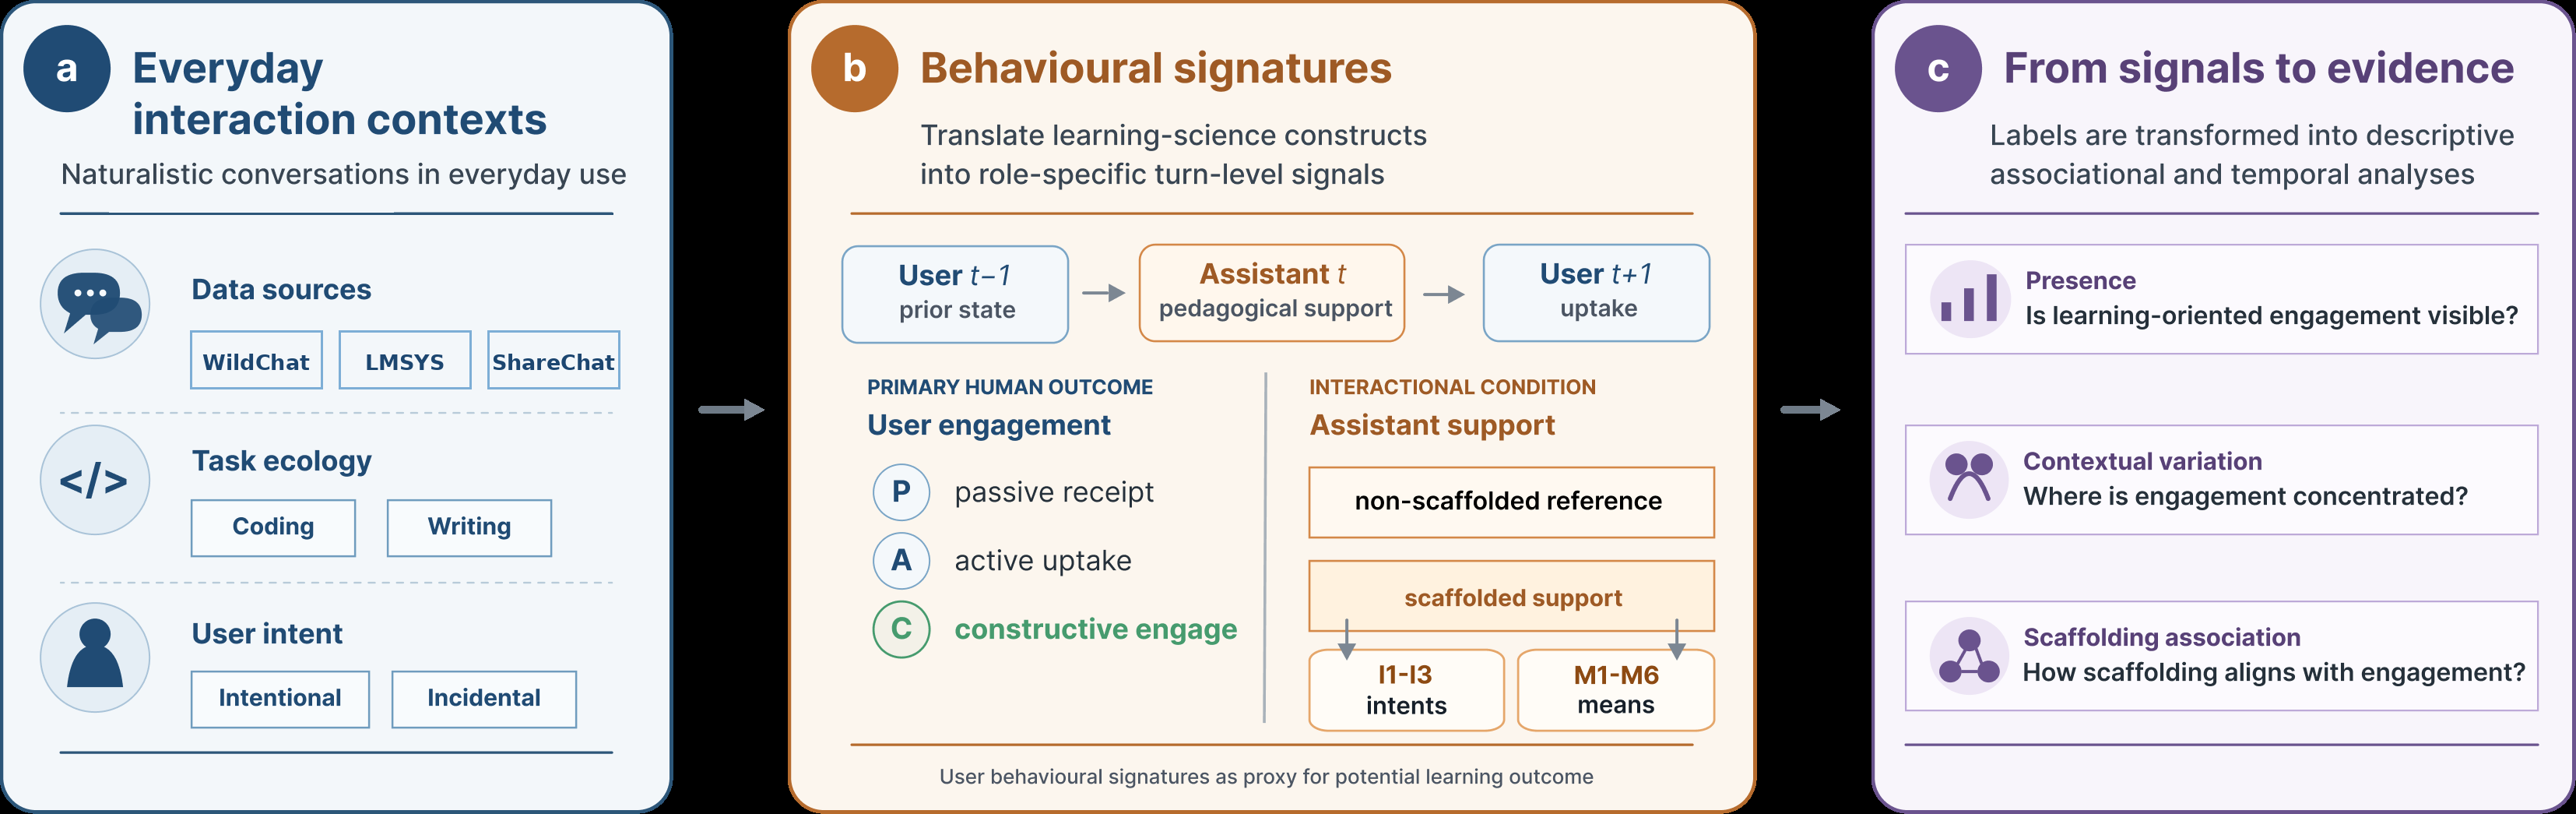
\includegraphics[width=\textwidth]{figures/figure_1_all_wild_lmsys.png}
\caption{
\textbf{Analytic framework for studying informal learning in everyday human--LLM interaction.}
\textbf{a,} Naturalistic public conversations are situated by task ecology and user framing.
\textbf{b,} Learning-science constructs are translated into turn-level behavioural signatures for user engagement and assistant support.
\textbf{c,} The resulting labels support analyses of engagement presence, contextual variation and scaffolding--engagement association. Labels capture observable interactional signatures, not durable learning outcomes or causal instructional effects.
}
    \label{fig:conceptual_framework}
\end{figure*}

\newpage

We find, first, that learning-oriented engagement is a recurrent feature of everyday human--LLM interaction, although its constructive form is selective. Across the three public corpora, cognitive engagement appears in 31.9\% of user turns and constructive engagement in 4.9\%, while emotional engagement is rare; scaffolded support appears in 31.7\% of assistant turns. These rates show that everyday AI use often involves more than answer delivery, but the deepest form of user engagement is a less frequent behavioural signal. Second, constructive engagement is organized by context: it is amplified by explicit learning framing, varies across task ecologies and becomes most visible in sustained exchanges where users return to, interrogate and reshape the assistant's response. Third, assistant scaffolding marks richer constructive participation across the six task settings, but not as a uniform or treatment-like effect. Its association with engagement depends on user framing, support form, task-specific support supply and temporal scale: feedback-like and explanatory support align most clearly with constructive engagement, whereas more directive or questioning forms are less aligned with visible elaboration, and the strongest temporal evidence is local, state-dependent and form-dependent rather than evidence for a uniform global trajectory. Together, these findings locate everyday human--LLM interaction in a middle space between ordinary tool use and designed instruction. By making this middle space observable, the study provides a foundation for future personal AI assistants that support lifelong learning in the flow of everyday work---not by turning every interaction into a formal lesson, but by helping everyday human--AI collaboration become a site where people build, test and extend understanding while solving real problems.
